\documentclass[a4paper,11pt]{article}
\author{ 杨旭鹏  \  PB17000234}
\date{2019年秋季}
\title{计算物理A 第十一题}

\usepackage{ctex}
\usepackage{amsmath}
\usepackage{amsfonts}
\usepackage{graphicx}
\usepackage{epstopdf}
\usepackage{lastpage}
\usepackage{hyperref}
\usepackage{listings}
\RequirePackage{xcolor}
\usepackage{appendix}
\usepackage{caption2}
\usepackage{subfigure}
\usepackage{float}
\usepackage{verbatim}
\makeatletter\def\@captype{table}\makeatother

\definecolor{dkgreen}{rgb}{0,0.6,0}
\definecolor{gray}{rgb}{0.5,0.5,0.5}
\definecolor{mauve}{rgb}{0.58,0,0.82}

\lstset{
  frame=tb,
  aboveskip=3mm,
  belowskip=3mm,
  showstringspaces=false,
  columns=flexible,
  framerule=1pt,
  rulecolor=\color{gray!35},
  backgroundcolor=\color{gray!5},
  basicstyle={\small\ttfamily},
  numbers=left,
  numberstyle=\tiny\color{gray},
  keywordstyle=\color{blue},
  commentstyle=\color{dkgreen},
  stringstyle=\color{mauve},
  breaklines=true,
  breakatwhitespace=true,
  tabsize=3,            
  }



\begin{document}
\maketitle
\tableofcontents

\section{题目描述}
数值研究 $d(d=1, 2, 3)$维空间中随机行走返回原点的几率步数$N$的变化关系 $P_{d}(N)$,能否定义相关的指数值?

\section{算法}

\subsection{指数定义}
我们不妨假设对于$P_{d}(N)$有$P_{d}(N) = a N^{\lambda}$,则有关系式:
\begin{equation}
	ln P_{d}(N) = \lambda ln N + ln a
\end{equation}


\subsection{一维情况}
设粒子在$t = 0$时刻从原点出发,向右移动的概率为$p_{+}$,向左移动的概率为$p_{-}$。则对于某位置$x$,行走$N$步后设粒子运动到此位置时向$x+$走了$n_{+}$步,$x-$走了$N-n_{+}$步,则有:
\begin{equation}
\begin{aligned}
	p_{N}(x) &= C_{N}^{n_{+}}p_{+}^{n_{+}}p_{-}^{N-n_{+}}  = \frac{N!}{n_{+}!(N-n_{+})!}p_{+}^{n_{+}}p_{-}^{N-n_{+}} \\
	&=  \frac{N!}{\frac{N+x}{2} !\frac{N-x}{2} !} p_{+}^{\frac{N+x}{2}}p_{-}^{\frac{N-x}{2}}
\end{aligned}
\end{equation}

可知$N+x,N-x$需为偶数,即$N,x$同奇偶。当返回原点时,即$x=0$时,$N$需要为偶数。此时有:
\begin{equation}
	P_{1}(N) = p_{N}(0) = \frac{N!}{\frac{N}{2}!\frac{N}{2}!}p_{+}^{\frac{N}{2}}p_{-}^{\frac{N}{2}}
\end{equation}

简单起见,假设粒子自由运动,$p_{+} = p_{-} = \frac{1}{2}$,则
\begin{equation}
	P_{1}(N) =   \frac{N!}{\frac{N}{2}!\frac{N}{2}!}\frac{1}{2^{N}}
\end{equation}

带入指数关系式得到:
\begin{equation}
\begin{aligned}
\lambda ln N + ln a &= ln \left(    \frac{N!}{\frac{N}{2}!\frac{N}{2}!}\frac{1}{2^{N}}    \right)	\approx ln \left(  \frac{\sqrt{2\pi N}(\frac{N}{e})^{N}}{\pi N (\frac{N}{2e})^{N}}  \frac{1}{2^{N}}   \right) \\
&= -\frac{1}{2}\left(  ln N + ln \pi -ln 2 \right)
\end{aligned}
\end{equation}

可知对于一维情况,当N比较大时,$P_{1}(N) \propto \frac{1}{\sqrt{N}}$。

\subsection{二维情况}
此时要求两个维度上均回到原点,利用同1维同样的思路得到:
\begin{equation}
	P_{2}(N) =   \sum_{i=0}^{\frac{N}{2}} C_{N}^{i}  C_{N-i}^{i} C_{N-2i}^{\frac{N-2i}{2}} \frac{1}{4^{N}}  =   \sum_{i=0}^{\frac{N}{2}} \frac{N!}{[i!(\frac{N}{2}-i)!]^{2}}\frac{1}{4^{N}} 
\end{equation}

发现指数不易得到,故二维及以上的指数可根据数值模拟结果进行拟合得到。

带入指数关系式中有:
\begin{equation}
\begin{aligned}
	\lambda ln N + ln a &= ln \left(   \sum_{i=0}^{\frac{N}{2}} \frac{N!}{[i!(\frac{N}{2}-i)!]^{2}}\frac{1}{4^{N}}    \right)
\end{aligned}
\end{equation}


\subsection{三维情况}
此时要求三个维度上均回到原点,利用同1维同样的思路得到:
\begin{equation}
\begin{aligned}
	P_{3}(N) &=  \sum_{i=0}^{\frac{N}{2}} \sum_{j=0}^{\frac{N}{2}-i} C_{N}^{i}  C_{N-i}^{i} C_{N-2i}^{j} C_{N-2i-j}^{j} C_{N-2i-2j}^{\frac{N-2i-2j}{2}} \frac{1}{6^{N}}  \\
	&=   \sum_{i=0}^{\frac{N}{2}} \sum_{j=0}^{\frac{N}{2}-i} \frac{N!}{[i!j!(\frac{N}{2}-i-j)!]^{2}}\frac{1}{6^{N}}
\end{aligned}
\end{equation}

同二维情况一样,三维情况的指数值同样需要数值模拟拟合得到。

\subsection{16807产生器}
作用中所产生的随机数使用16807产生器产生。16807产生器属于线性同余法产生器的特例。而线性同余法方法为:

\begin{equation}
\begin{aligned}
	I_{n+1} &= (aI_{n} + b) \ mod \ m \\
	x_{n} &= I_{n}/m
\end{aligned}
\label{linear}	
\end{equation}

其中整数$I_{i} \in [0,m-1]$,$a,b,m$为算法中的可调参数,其选取直接影响产生器的质量。选取参数:
\begin{equation}
\left\{
\begin{array}{l}
	a = 7^{5} = 16807 \\
	b = 0 \\
	m = 2^{31}-1 = 2147483647
\end{array}
\right.
\end{equation}

即为所谓的16807产生器。由于直接利用\ref{linear}编写程序时计算$(aI_{n} \ mod \ m )$时很容易造成数据溢出,故采取Schrage方法进行具体编程的实现:

\begin{equation}
	aI_{n} \ mod \ m = \left\{
	\begin{array}{l}
		a(I_{n}\ mod \ q) - r[I_{n}/q],\ \ \ \ \ \ \ \ if \geq 0 \\
		a(I_{n}\ mod \ q) - r[I_{n}/q] + m,\ \ otherwise	
			\end{array}
	\right.
\end{equation}

其中$m=aq+r$,即$q=m/a=127773$,$r=m \ mod \ a=2836$。即可利用此方法产生伪随机数序列。
\subsection{RW算法简述}

对于$n$维情况,对于每一个粒子先利用16807产生器产生一组均匀分布在$[0,1]$的随机数,对于此粒子的第$k$步来说,若第$k$个随机数$\in (0,\frac{1}{n}]$,则向x轴正方向走一个单位长度;若$\in (\frac{1}{n},\frac{2}{n}]$,向x轴负向走一个单位;若$\in (\frac{2}{n},\frac{3}{n}]$,向y轴正向走一个单位;若$\in (\frac{3}{n},\frac{4}{n}]$,向y轴负向走一个单位;若$\in (\frac{4}{n},\frac{5}{n}]$,向z轴正向走一个单位;若$\in (\frac{5}{n},1]$,向z轴负向走一个单位。行走共$N$步后,查看其位置坐标是否为原点,是的话计数器$+\frac{1}{n}$,则进行$n$个粒子模拟后,计数器的值即为数值模拟得到的近似$N$步回到原点的概率。


\section{程序使用方法}
在运行程序后,会看到请求输入所需计算的随机行走的总步数,按照提示在后面输入,摁回车继续。屏幕请求输入进行模拟的总粒子数,输入后摁回车继续。然后程序会将三个维度不同步数所对应的回到原点的概率输出至文件。程序输出完这些后会自动退出。

\begin{figure}[!htbp]        
\centering

\includegraphics[width=7cm]{example.png}      
\caption{ 一个典型程序的运行示例}      
\end{figure}


\section{程序结果与讨论}
当我们选取$n=10^{5}$时,模拟100步得到结果:

\begin{figure}[!htbp]        
\centering
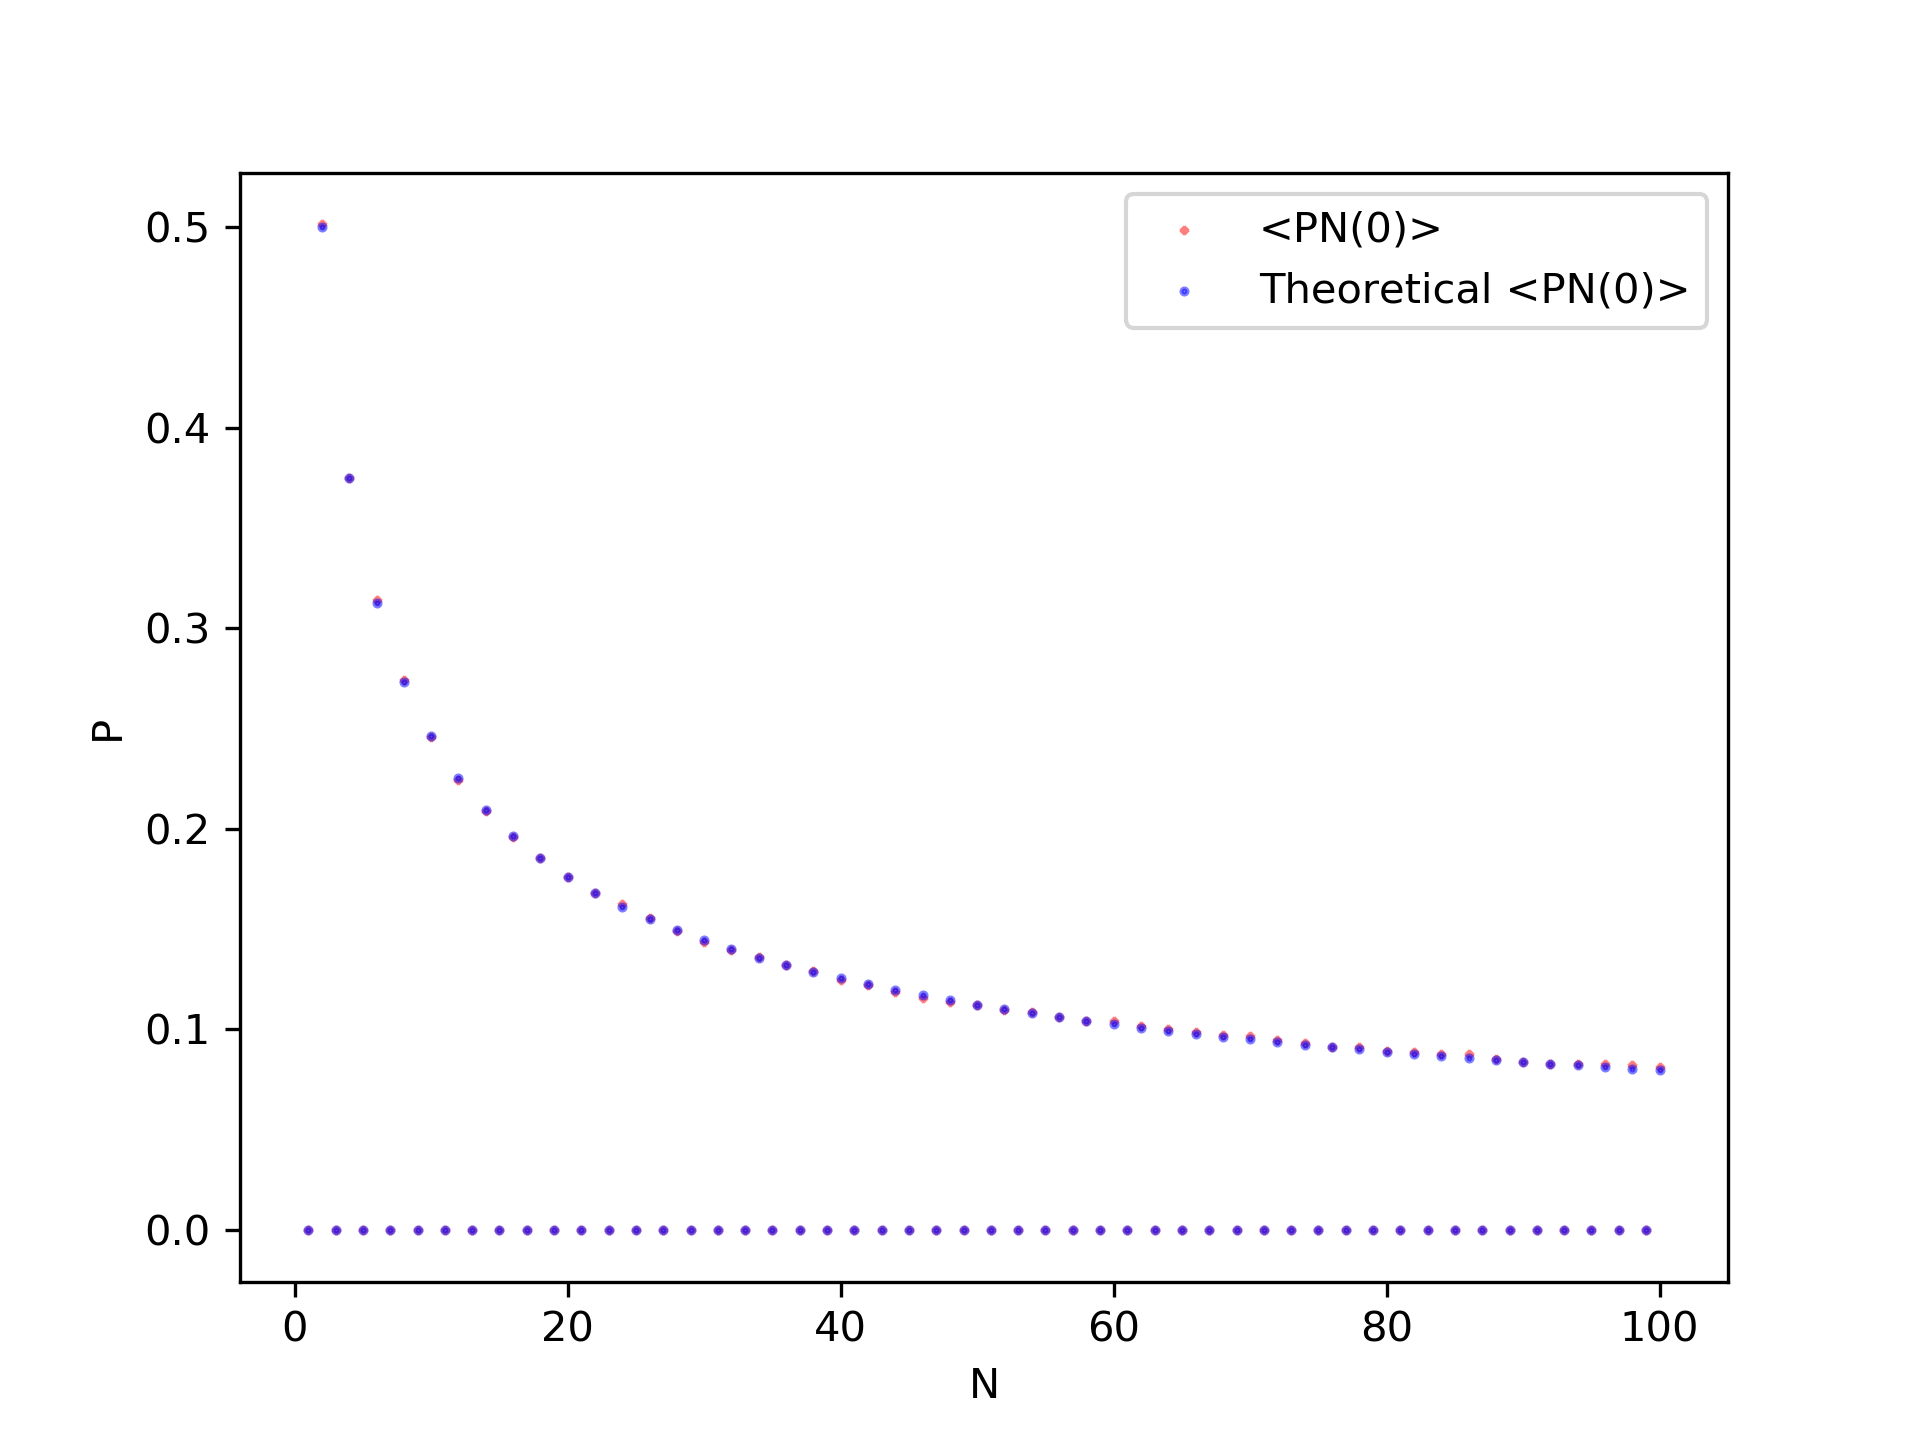
\includegraphics[width=9cm]{1-105.png}      
\caption{一维下$n=10^{5}$,$N=100$时回到原点的概率与步数的关系散点图}      
\end{figure}


\begin{figure}[!htbp]        
\centering
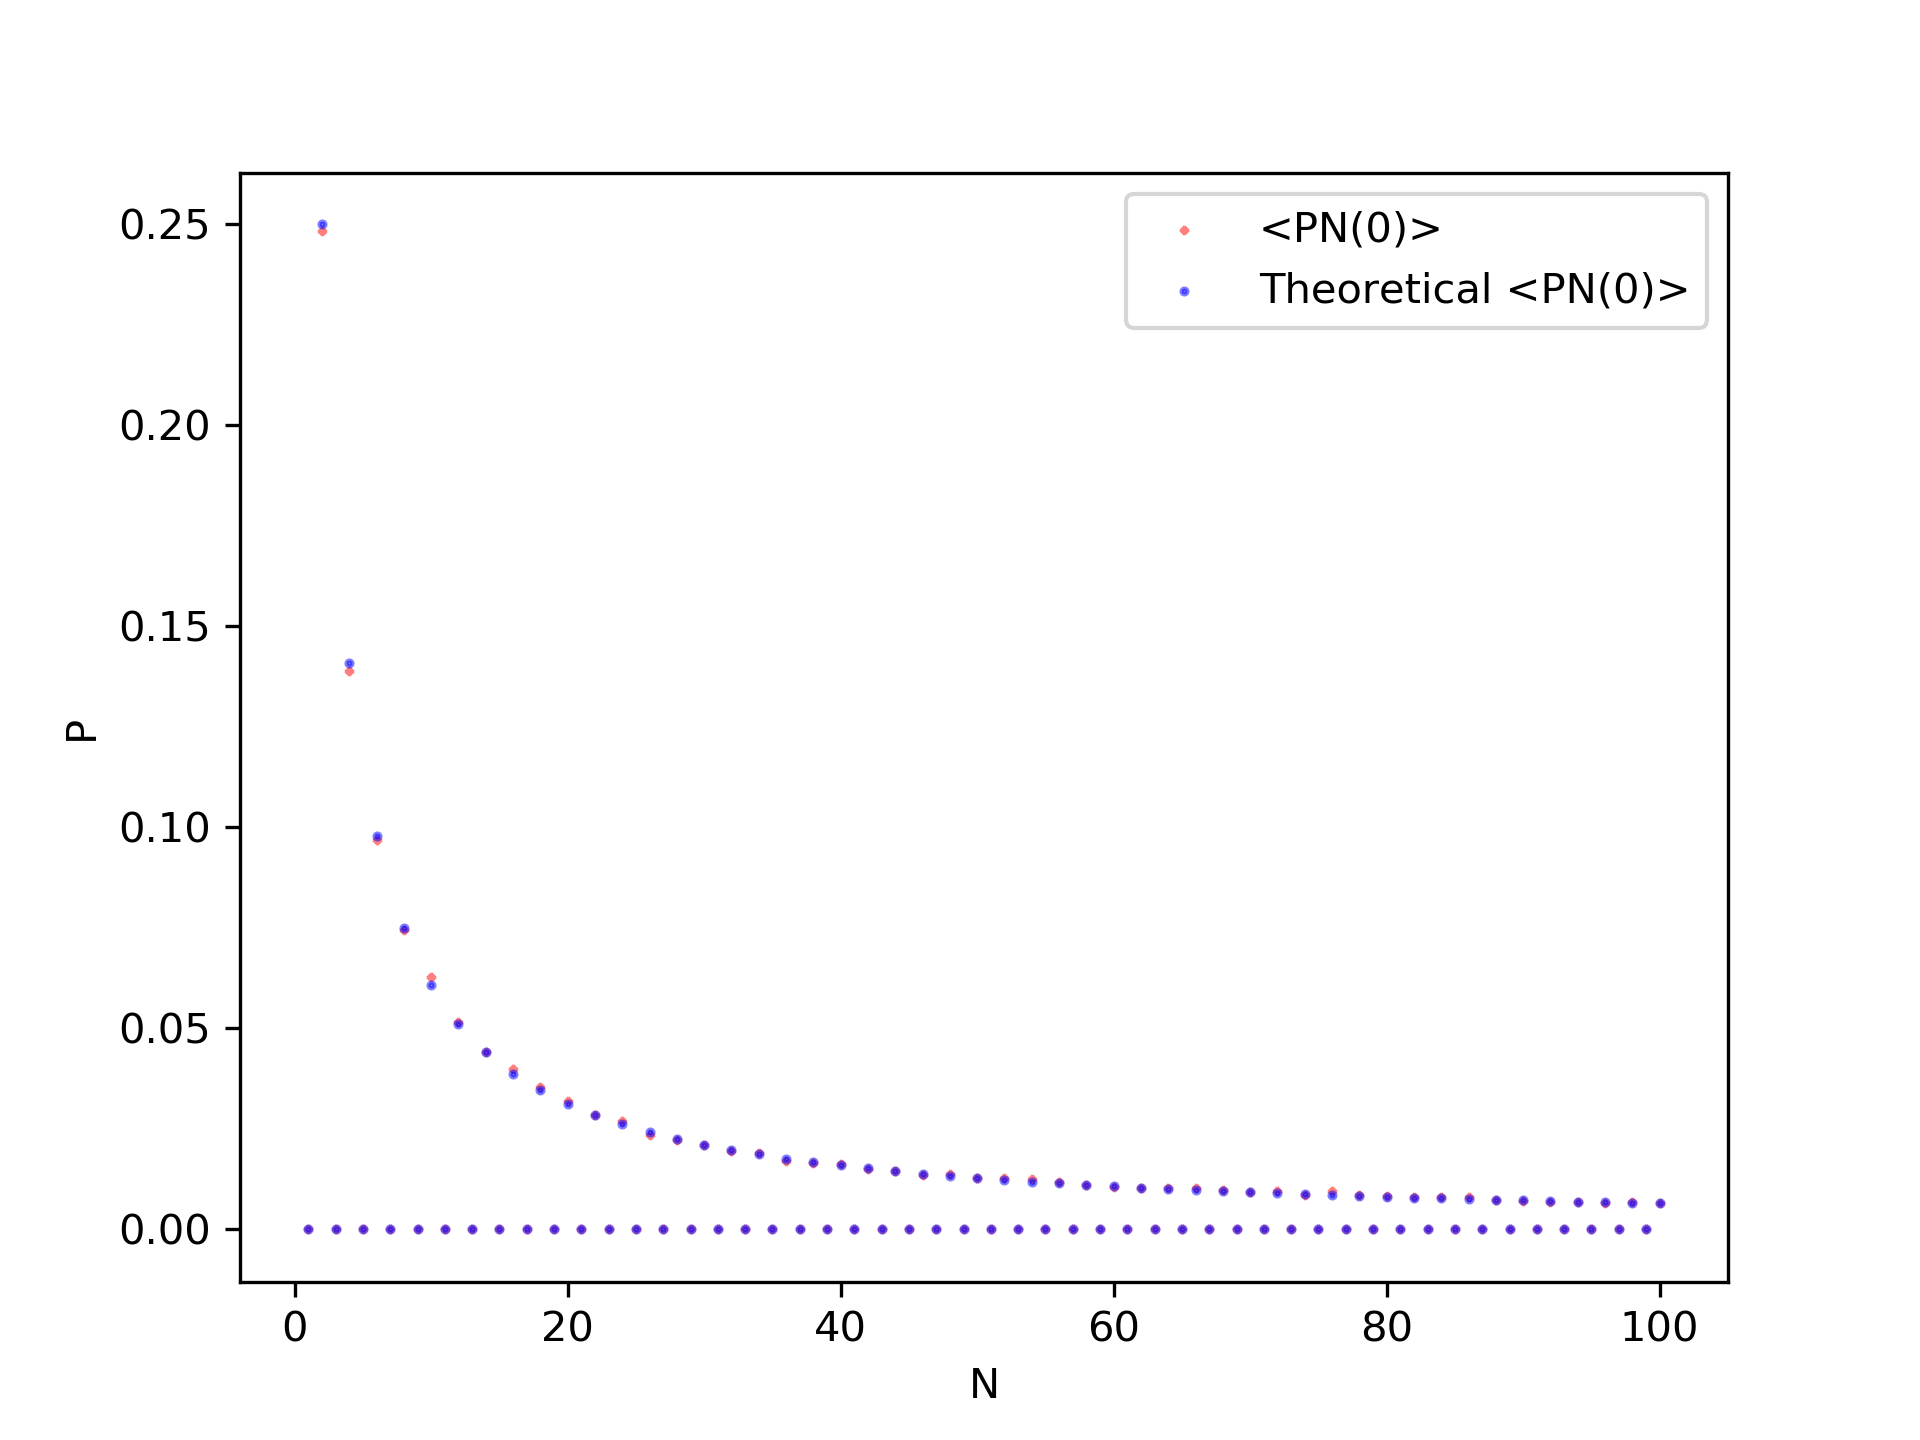
\includegraphics[width=9cm]{2-105.png}      
\caption{ 二维下$n=10^{5}$,$N=100$时回到原点的概率与步数的关系散点图}      
\end{figure}


\begin{figure}[!htbp]        
\centering
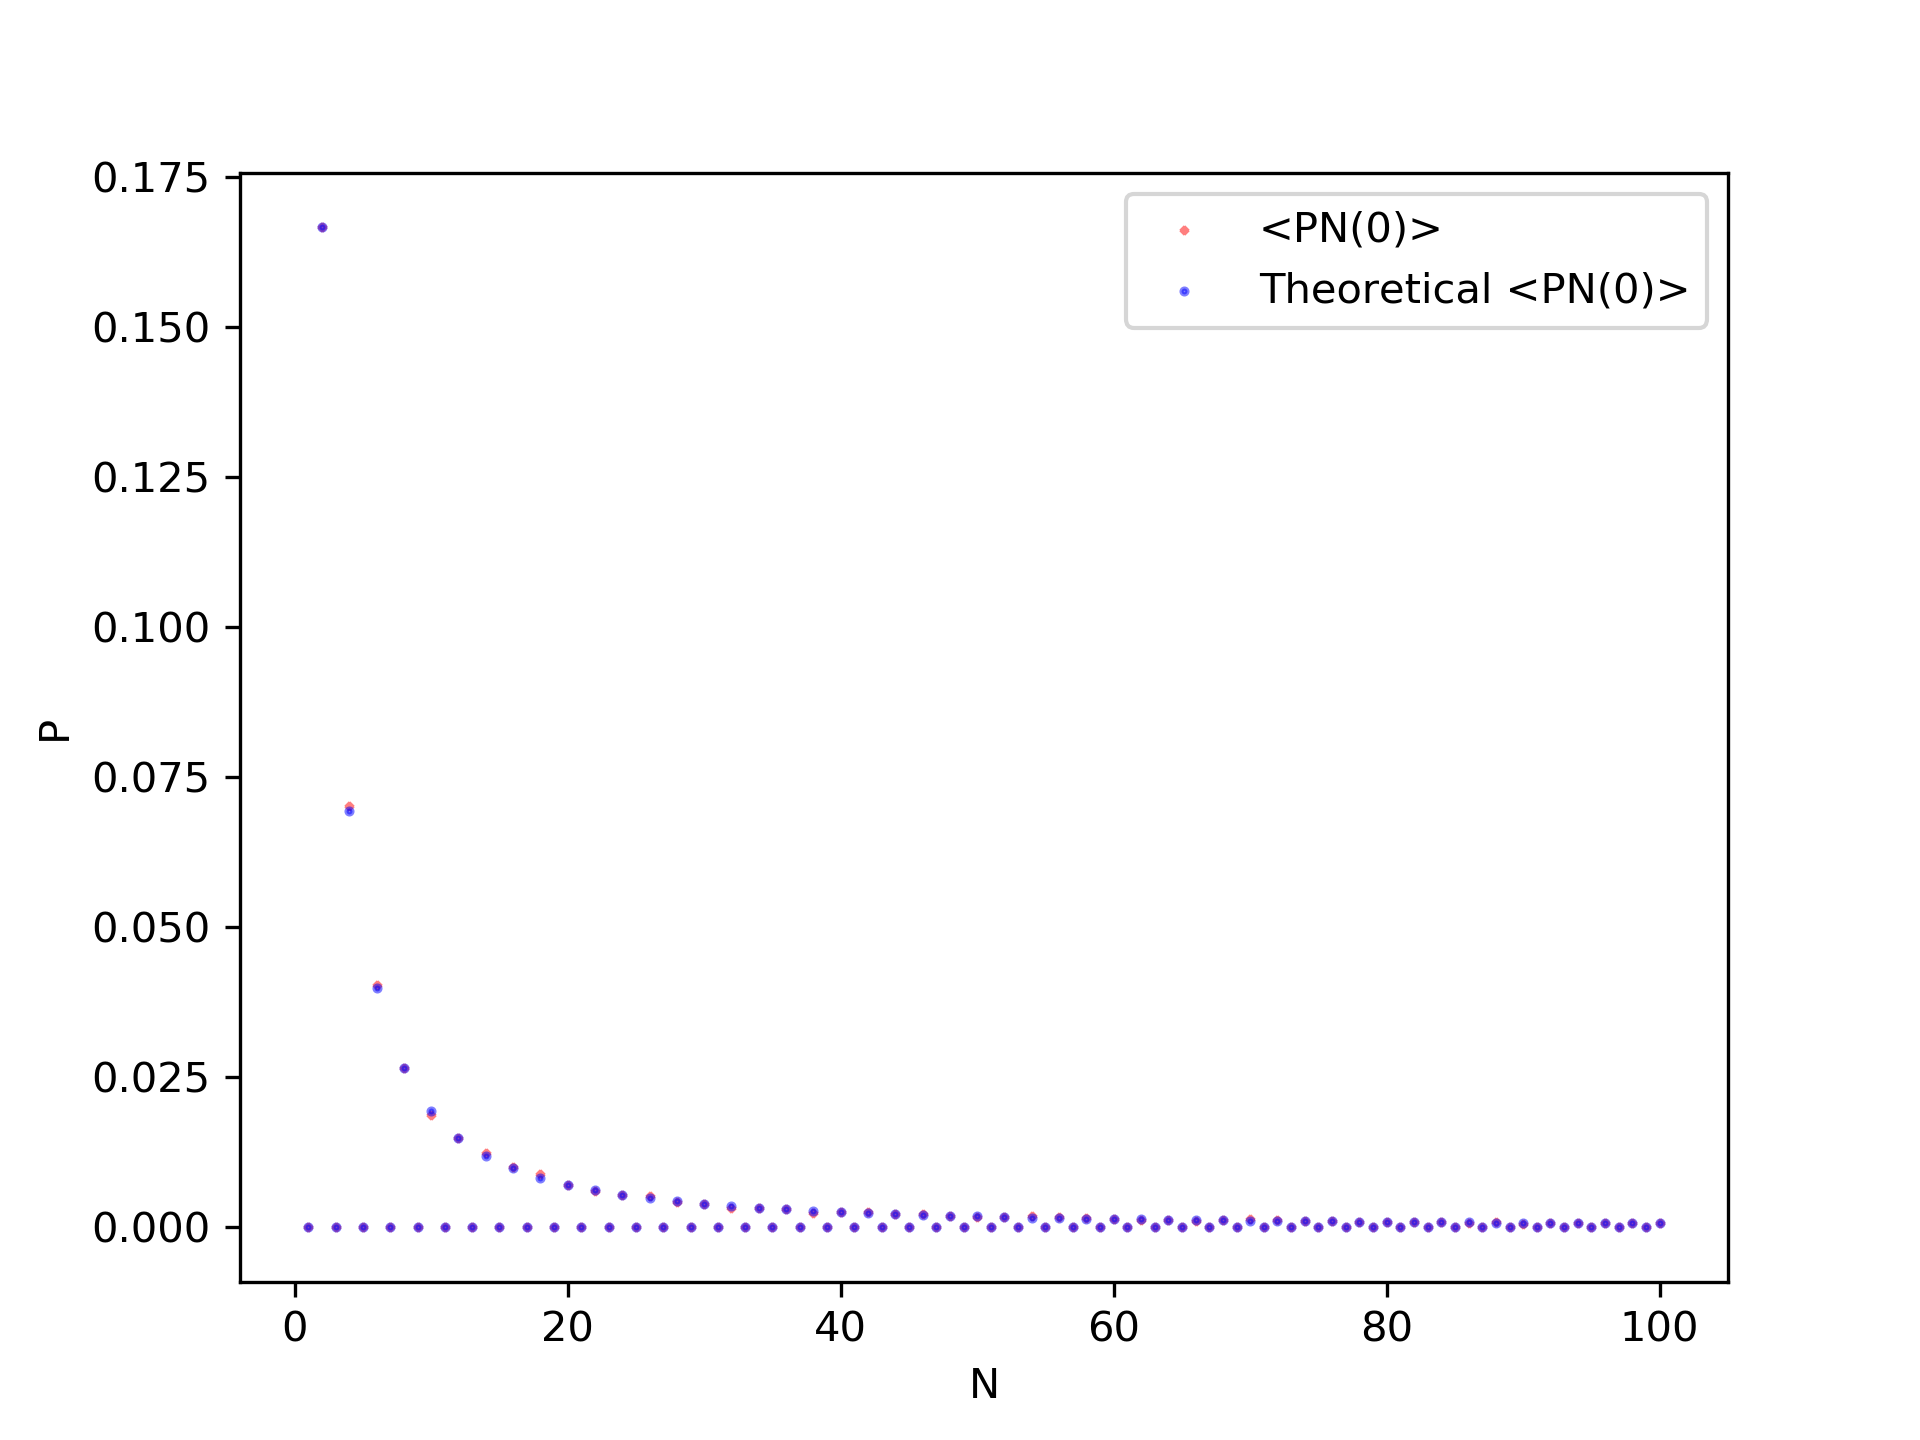
\includegraphics[width=9cm]{3-105.png}      
\caption{ 三维下$n=10^{5}$,$N=100$时回到原点的概率与步数的关系散点图}      
\end{figure}
	


\newpage
可以看出数值模拟结果和理论值基本一致,基本验证了理论概率关系。
为了得到指数关系,我们利用Python脚本\footnote{具体脚本见附录}将不同维度得到的数据进行对数操作并进行线性拟合得到如下结果:

\begin{table}[!htbp]
\centering
\resizebox{\textwidth}{!}{
\begin{tabular}{|c|c|c|c|}
\hline
&一维情况&二维情况&三维情况 \\ \hline
线性拟合系数$\lambda$&-0.49621484  &-0.99203304   &-1.49448087 \\ \hline
拟合截距 $ln a$ &-0.24924804  &-0.49986808  &-0.46930788 \\ \hline
\end{tabular}}
\caption{$n=10^{6}$,$N=1000$时不同维度的线性拟合结果}
\end{table}

根据数据进行猜测,可能对于比较大的$N$有:
\begin{table}[!htbp]
\centering
\resizebox{\textwidth}{!}{
\begin{tabular}{|c|c|c|c|}
\hline
&一维情况&二维情况&三维情况 \\ \hline
猜测的结果& $P_{1}(N) \propto \frac{1}{\sqrt{N}} $ & $P_{2}(N) \propto \frac{1}{N}$  & $P_{3}(N) \propto N^{-\frac{3}{2}}$ \\ \hline
\end{tabular}}
\caption{不同维度的指数关系猜测}
\end{table}

上面的结果即为:
\begin{equation}
	P_{d}(N) \propto N^{-\frac{d}{2}}
\end{equation}

结合数值模拟结果能说明:
\begin{description}
\item[1] $N$为奇数时,1维、2维、3维返回原点概率都为0
\item[2]随着$N$增⼤,1维、2维、3维返回原点概率$P_{d}(N)$都减⼩
\item[3]相同步数$N$的情况下,维数$d$越⼤,返回原点的概率越⼩,趋于$0$速度越快
\end{description}


\section{心得与体会}
通过此次作业,对随机行走的一些规律及特征有了更深刻的认识。


\newpage
\section{附录}

\begin{appendices}


\section{C语言源程序}
\begin{lstlisting}[language = C]
#include <stdio.h>
#include <stdlib.h>
#include <math.h>
#include <string.h>
#define a 16807
#define b 0
#define m 2147483647
#define r (m%a)
#define q (m/a)
#define Pi 3.1415926
#define round(x) ((x)>=0?(int)((x)+0.5):(int)((x)-0.5))


//利用/dev/random 产生"真"随机数
int my_realrandom(int ran[],int n){
    FILE *fp1 = fopen("/dev/random","r");
    for(int i=0;i<n;i++){
        fread(&ran[i], 1, 4, fp1);
    }
    fclose(fp1);
    return 0;
}



int my_filewriter_double(char str1[],char str2[],double num,int flag){
    FILE * fp;
    char str[20];
    strcpy(str,str1);
    strcat(str,str2);
    fp = fopen(str,"a+");

    if(flag == 1) fprintf(fp,"%lf",num);    //最后一个数据后不加 ","
    else fprintf(fp,"%lf,",num);
    
    fclose(fp);
    return 0;
}


// Schrage 方法产生随机数
int my_schrage(double ran[],int seed,int n){
    for (int i = 0; i < n - 1; i++) {
        if (seed >= 0) {
            ran[i] = (seed / (double) m);
        } else {
            ran[i] = ((seed + m) / (double) m);
        }
        if(seed == m-1){
            if(a >=  b){    //由于Schrage方法只对z in (0,m-1)成立,故这里要讨论z == m-1的情况
                seed = m + (b-a) % m;
            }
            else   seed =  (b-a) % m;

        }
        else seed = ((a * (seed % q) - r * (seed /  q)) + b % m ) % m;  //递推式
        
        
    }
    if (seed >= 0) {
        ran[n-1] = (seed / (double) m);
    } else {
        ran[n-1] = ((seed + m) / (double) m);
    }
    return 0;
}

int num2str(char str[],int num){
    int  n, i = 0;
    char tmp[20];
    n = num % 10;
    while (n>0 || num > 0)
    {
        tmp[i++] = n + '0';
        num = (num - n) / 10;
        n = num % 10;
    }
    tmp[i] = '\0';
    for (i=0; i<=strlen(tmp)-1; i++)
    {
        str[i] = tmp[strlen(tmp)-i-1];
    }
    str[i] = '\0';
    return 0;
}



// Schrage 方法RW
int my_schrage_1DRW(double ran[],int N,int x[]){ //一维随机行走
    for(int i =0;i<3;i++){ //位置坐标初始化
        x[i] = 0;
    }
    
    for (int i = 0; i < N; i++) {
        if (ran[i] < 0.5) x[0] += -1;
        else x[0] += 1;
    }
    return 0;
}


int my_schrage_2DRW(double ran[],int N,int x[]){ //二维随机行走
    for(int i =0;i<3;i++){ //位置坐标初始化
        x[i] = 0;
    }
    
    for (int i = 0; i < N; i++) {
        if (ran[i] < 0.25) x[0] -= 1;
        else if((ran[i] < 0.5) && (ran[i] >= 0.25)) x[0] += 1;
        else if((ran[i] < 0.75) && (ran[i] >= 0.5)) x[1] -= 1;
        // if(ran[i] >= 0.75 && ran[i] < 1 ) x[1] += 1;
        else x[1] += 1;
    }
    return 0;
}

int my_schrage_3DRW(double ran[],int N,int x[]){   //三维随机行走
    for(int i =0;i<3;i++){ //位置坐标初始化
        x[i] = 0;
    }
    
    for (int i = 0; i < N; i++) {
        if (ran[i] < (double)1/6 ) x[0] -= 1;
        else if(ran[i] < (double)1/3 && ran[i] >= (double)1/6) x[0] += 1;
        else if(ran[i] < (double)1/2 && ran[i] >= (double)1/3) x[1] -= 1;
        else if(ran[i] < (double)2/3 && ran[i] >= (double)1/2) x[1] += 1;
        else if(ran[i] < (double)5/6 && ran[i] >= (double)2/3) x[2] -= 1;
        else x[2] += 1;
    }
    return 0;
}


int main(int argc, const char * argv[]) {
    int N;    //步长最大值
    int n;    //总粒子个数
    char str[50];
    printf("请输入您所需要的步数最大值:");
    while (!scanf("%d",&N)){   //简单的输入检查
        gets(str);
        printf("\nInput error,please try again\n");
        printf("请输入您所需要的步数最大值:");
    }
    
    printf("请输入您所需总粒子个数:");
    while (!scanf("%d",&n)){   //简单的输入检查
        gets(str);
        printf("\nInput error,please try again\n");
        printf("请输入您所需要的总粒子个数:");
    }
    
    if(N*n >1000000) printf("您输入的参数已接受,正在计算请稍等片刻~\n");

    double *ran = malloc(sizeof(double) * N);  //用来存放每个粒子每一步的位置
    int *seed = malloc(sizeof(int) * n);  //用来存放随机种子值
    double p[3]; //存放3个维度返回原点的概率
    int x[3];   //存放粒子最后的坐标值
    
    my_realrandom(seed, n);  //产生随机种子
    
    char str1[10];
    int flag = 0;  //是否为最后一个数据(j=N)的标志
    num2str(str1, N);
    
    for(int j = 1; j<=N ;j++){  //j为步数
        
        for(int i = 0;i<3;i++){  //概率初始化置零
            p[i] = 0;
        }
        
        for(int i=0;i<n;i++){  //i为粒子个数
            my_schrage(ran, seed[i], j);
            my_schrage_1DRW(ran, j, x);
            if(x[0] == 0) p[0] += (double) 1/n;
            my_schrage_2DRW(ran, j, x);
            if((x[0] == 0) && (x[1] == 0) ) p[1] += (double) 1/n;
            my_schrage_3DRW(ran, j, x);
            if(x[0] == 0 && x[1] == 0 && x[2] == 0 ) p[2] += (double) 1/n;
        }
        if (j == N) flag = 1;
        my_filewriter_double(str1, "step-1p.txt", p[0], flag);
        my_filewriter_double(str1, "step-2p.txt", p[1], flag);
        my_filewriter_double(str1, "step-3p.txt", p[2], flag);
    }
    
        
    return 0;
}

\end{lstlisting}

\newpage

\section{可视化绘图及数据处理Python程序源码}

\begin{lstlisting}[language = python]
import matplotlib.pyplot as plt
import numpy as np
import math
plt.rcParams['savefig.dpi'] = 300 #图片像素
plt.rcParams['figure.dpi'] = 300 #分辨率
# 默认的像素:[6.0,4.0],分辨率为100,图片尺寸为 600&400
fig1 = plt.figure()
fig1t = plt.figure()
fig2 = plt.figure()
fig3 = plt.figure()

ax1 = fig1.add_subplot(111)
ax1t = fig1t.add_subplot(111)
ax2 = fig2.add_subplot(111)
ax3 = fig3.add_subplot(111)


N = 100   # 每个粒子行走的步数N
n = 6     # 模拟的粒子数量,单位为10^n
X = []    # 存储步数N
Y1 = []   # 存储一维每一步回到原点的概率
Y2 = []   # 存储二维每一步回到原点的概率
Y3 = []   # 存储三维每一步回到原点的概率
Yt1 = np.zeros(N)   # 存储一维每一步回到原点的理论概率
Yt2 = np.zeros(N)   # 存储二维每一步回到原点的理论概率
Yt3 = np.zeros(N)   # 存储三维每一步回到原点的理论概率

with open('problem 11/100step-1p_10'+str(n)+'.txt', 'r') as f:
    while True:
        lines = f.readline() # 整行读取数据
        if not lines:
            break
        Y1 = [float(i) for i in lines.split(',')]  # 将整行数据分割处理
    Y1 = np.array(Y1) # 将数据从list类型转换为array类型。

with open('problem 11/100step-2p_10'+str(n)+'.txt', 'r') as f:
    while True:
        lines = f.readline() # 整行读取数据
        if not lines:
            break
        Y2 = [float(i) for i in lines.split(',')]  # 将整行数据分割处理
    Y2 = np.array(Y2) # 将数据从list类型转换为array类型。


with open('problem 11/100step-3p_10'+str(n)+'.txt', 'r') as f:
    while True:
        lines = f.readline() # 整行读取数据
        if not lines:
            break
        Y3 = [float(i) for i in lines.split(',')]  # 将整行数据分割处理
    Y3 = np.array(Y3) # 将数据从list类型转换为array类型。


X = np.arange(1, N+1, 1)  # 每一步的数值N


for i in range(N):   # 计算一维情况下理论上每一步对应的回到原点的概率
    if (i+1) % 2 == 0:
        Yt1[i] = math.factorial((i+1))/(pow(math.factorial((i+1)/2), 2))*pow(0.5, (i+1))  
    else:
        Yt1[i] = 0

for i in range(N):   # 计算二维情况下理论上每一步对应的回到原点的概率
    if (i+1) % 2 == 0:
        for j in range(round((i+1)/2)+1):
            Yt2[i] += math.factorial(i+1)/pow(math.factorial(j)*math.factorial(round((i+1)/2)-j), 2)*pow(1./4, (i+1))
    else:
        Yt2[i] = 0

for i in range(N):  # 计算三维情况下理论上每一步对应的回到原点的概率
    if (i+1) % 2 == 0:
        for j in range(round((i+1)/2)+1):
            for k in range(round((i+1)/2)-j+1):
                Yt3[i] += math.factorial(i + 1) / (pow(math.factorial(j) * math.factorial(k) * math.factorial(round((i + 1) / 2) - j - k), 2)) * pow(
                    1./6, (i + 1))
    else:
        Yt3[i] = 0


ax1.scatter(X, Y1, c='r', label='<PN(0)>', s=2, alpha=0.5, marker='x')   # 一维情况下每一步对应的回到原点的概率散点图 数值模拟VS理论
ax1.scatter(X, Yt1, c='b', label='Theoretical <PN(0)>', s=2, alpha=0.5)
ax1.set_xlabel('N')
ax1.set_ylabel('P')
ax1.legend(loc=1)
fig1.savefig("1.png")


ax2.scatter(X, Y2, c='r', label='<PN(0)>', s=2, alpha=0.5, marker='x')   # 二维情况下每一步对应的回到原点的概率散点图 数值模拟VS理论
ax2.scatter(X, Yt2, c='b', label='Theoretical <PN(0)>', s=2, alpha=0.5)
ax2.set_xlabel('N')
ax2.set_ylabel('P')
ax2.legend(loc=1)
fig2.savefig("2.png")


ax3.scatter(X, Y3, c='r', label='<PN(0)>', s=2, alpha=0.5, marker='x')   # 三维情况下每一步对应的回到原点的概率散点图 数值模拟VS理论
ax3.scatter(X, Yt3, c='b', label='Theoretical <PN(0)>', s=2, alpha=0.5)
ax3.set_xlabel('N')
ax3.set_ylabel('P')
ax3.legend(loc=1)
fig3.savefig("3.png")

for i in range(50):   # 将每个维度上奇数步概率为0的数据删掉
    X = np.delete(X, i)
    Y1 = np.delete(Y1, i)
    Y2 = np.delete(Y2, i)
    Y3 = np.delete(Y3, i)

print(np.polyfit(np.log(X), np.log(Y1), 1))   # 对每一维度上的指数值进行线性拟合
print(np.polyfit(np.log(X), np.log(Y2), 1))
print(np.polyfit(np.log(X), np.log(Y3), 1))

\end{lstlisting}


\end{appendices}




\end{document}
